\chapter{Instrumentation with ScoreP}
\label{cha:scorep}

\section{Introduction}

Parallel computing can be complex when working with large programs. In order to
get a better overview of a programs behavior and possible inefficiencies, many
instrumentation packages have been produced to aid developers in finding
bottlenecks in their code. Instrumentation refers the insertion of pragmas into
an existing code the monitor the codes behavior at runtime and saves a record
for latter review. Although instrumentation can be useful, it should be noted
that when instrumentation is inserted into code, it may cause changes in
performance. These changes can be due to changes in memory allocation due to
the instrumentation's presence and can also cause Heisenbugs, or the change in
a program's behavior when trying to observer it. The two main types of
instrumentation are profiling and tracing. Profiling describes the measurement
of the duration or frequency of function calls. This can be very useful in
gaining an overview of a programs characteristic, and discovering
computationally intensive hotspots. Profiling is fairly inexpensive and can
provide a moderate amount of performance data. What profiling does not excel in
is displaying the chronological order of events relative to one another. For
this purpose, tracing is better suited. Tracing can be used to recreate and
study dynamic program behavior after program execution has completed. Tracing
logs event information about a programs execution and communication at run
time. Events usually consist of timestamps and process ids as well as process
specific data. These event logs can be very large in size and are written to a
memory buffer during execution, and must be flushed (written to disk) when the
buffers fill. For this reason, tracing can more heavily influence the execution
of program when improperly implemented. Both tracing and profiling can be
helpful when looking to find performance bottlenecks in parallel code, and when
used together can be very powerful. One large instrumentation package developed
in Germany is ScoreP.

ScoreP is a compiler wrapper that allows developers to take advantage of
multiple instrumentation tool like Vampir, Cube, and Scalasca while using only
one compiler wrapper. By setting environment variables, the user can easily turn
functionalities on and off at runtime.

\section{Goals and approach}

Our goals for our code analysis were to identify excessive communication,
frequent synchronization and load balancing issues. To analyzing our code, we
first profiled the code and analyzed the results in Cube. This allowed us to get
an overview of the computationally intensive processes and assess weather or not
we would like to filter out. When not using a filter file, the flush points were
manageable for low scale simulations but became more disturbing as the
simulations became large. We then implemented a filter for the Petsc solve
directory to solve this issue.

We were then able to confidently activate tracing and run another
simulation. When viewing the trace data in figure \ref{fig:scorep-trace-data},
one can see that after MPI initialization, the computational intensity of our
simulation is relatively high. The largest load-imbalance and synchronization
issue when calling MPI allreduce, which arises on vtk write iterations.

\begin{figure}[h]
  \centering
  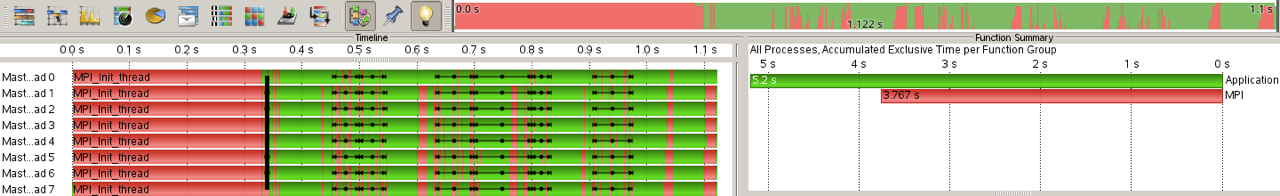
\includegraphics[width=\textwidth]{FIGURES/scorep/trace-data}
  \caption{Nodes waiting for one another during VTK output}
  \label{fig:scorep-trace-data}
\end{figure}

This can most likely be attributed to the bottleneck at the disk when outputting
the VTK files. This phenomenon was removed after the vtk output was
deactivated. With the VTK output turned off, the computational intensity was
consistently high.

\begin{figure}[h]
  \centering
  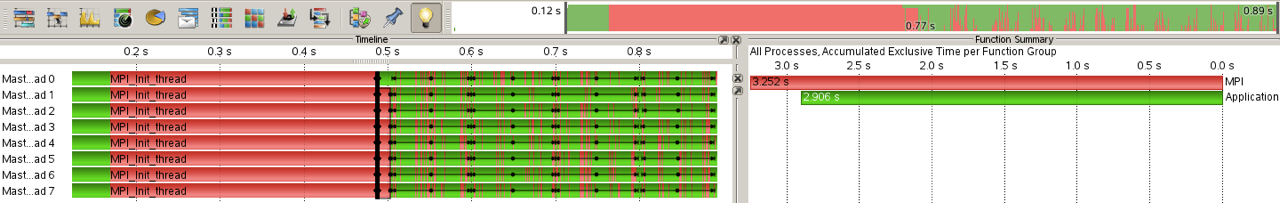
\includegraphics[width=\textwidth]{FIGURES/scorep/reference}
  \caption{Trace showing high computational intensity}
  \label{fig:scorep-reference}
\end{figure}

This could be supplemented with a parallel file access system which was not
present during this simulation. With figure \ref{fig:scorep-reference} the rest
of the computation has a considerably high computational intensity, that we are
very pleased with.
